\documentclass[10pt]{ctexart}
\usepackage{listings}
\usepackage{amsmath} 
\usepackage{amssymb} 
\usepackage{xcolor}
\usepackage{xeCJK}
\usepackage{fontspec}
\usepackage{titlesec}
\usepackage{titletoc}
\usepackage{setspace}
\usepackage{graphicx}
\usepackage{geometry}
\usepackage[T1]{fontenc}  
\usepackage{textcomp}
\usepackage{lmodern}
%\usepackage{caption}
\usepackage[justification=centering]{subcaption}
\usepackage[justification=centering]{caption}
\usepackage{tikz}
\usetikzlibrary{graphs}
\usepackage{amsfonts}
\usepackage[colorlinks,
            linkcolor=black,
            anchorcolor=black,
            citecolor=black]{hyperref}
\geometry{a4paper,scale=0.8}
\renewcommand\contentsname{Contents}
%\setmonofont[Mapping={}]{Monaco}    %英文引号之类的正常显示,相当于设置英文字体
%\setsansfont{Consolas} %设置英文字体 Monaco, Consolas,  Fantasque Sans Mono
%\setmainfont{Monaco} %设置英文字体
\setmonofont{Consolas}
% 定义可能使用到的颜色
%\setmainfont[BoldFont=SimHei]{SimSun}
\definecolor{CPPLight}  {HTML} {686868}
\definecolor{CPPSteel}  {HTML} {888888}
\definecolor{CPPDark}   {HTML} {262626}
\definecolor{CPPBlue}   {HTML} {4172A3}
\definecolor{CPPGreen}  {HTML} {487818}
\definecolor{CPPBrown}  {HTML} {A07040}
\definecolor{CPPRed}    {HTML} {AD4D3A}
\definecolor{CPPViolet} {HTML} {7040A0}
\definecolor{CPPGray}  {HTML} {B8B8B8}
\lstset{
    columns=fixed,       
    % numbers=left,                                        % 在左侧显示行号
    frame=none,                                          % 不显示背景边框
    backgroundcolor=\color[RGB]{245,245,244},            % 设定背景颜色
    keywordstyle=\color[RGB]{40,40,255},                 % 设定关键字颜色
    numberstyle=\small\color{darkgray},                  % 设定行号格式
    commentstyle=\it\color[RGB]{0,96,96},                % 设置代码注释的格式
    stringstyle=\rmfamily\slshape\color[RGB]{128,0,0},   % 设置字符串格式
    showstringspaces=false,                              % 不显示字符串中的空格
    language=c++,                                        % 设置语言
    morekeywords={alignas,continute,friend,register,true,alignof,decltype,goto,
    reinterpret_cast,try,asm,defult,if,return,typedef,auto,delete,inline,short,
    typeid,bool,do,int,signed,typename,break,double,long,sizeof,union,case,
    dynamic_cast,mutable,static,unsigned,catch,else,namespace,static_assert,using,
    char,enum,new,static_cast,virtual,char16_t,char32_t,explict,noexcept,struct,
    void,export,nullptr,switch,volatile,class,extern,operator,template,wchar_t,
    const,false,private,this,while,constexpr,float,protected,thread_local,
    const_cast,for,public,throw,std},
    emph={map,set,multimap,multiset,unordered_map,unordered_set,
    unordered_multiset,unordered_multimap,vector,string,list,deque,
    array,stack,forwared_list,iostream,memory,shared_ptr,unique_ptr,
    random,bitset,ostream,istream,cout,cin,endl,move,default_random_engine,
    uniform_int_distribution,iterator,algorithm,functional,bing,numeric,},
    emphstyle=\color{CPPViolet},
    basicstyle=\linespread{1}\small\fontspec{Consolas}\ttfamily,
    breaklines=true,
    %xleftmargin=1em,xrightmargin=1em, aboveskip=1em,
    % in the listings package configuration, try:  
    literate={"}{\textquotedbl}1,  
    tabsize=4, keepspaces=true
}
\CTEXoptions[today=old]
\title{Exercises 5}
\author{软件工程一班 \ 张逸松 57号}
\date{\today}

\begin{document}
    \maketitle
    \subsection*{1.2}
        \begin{itemize}
            \item [\textbf{a)}] It's not reflexive, not symmetric, not antisymmetric, transitive.
            \item [\textbf{b)}] It's reflexive, symmetric, not antisymmetric, transitive.
            \item [\textbf{c)}] It's not reflexive, symmetric, not antisymmetric, not transitive.
            \item [\textbf{d)}] It's not reflexive, not symmetric, antisymmetric, transitive.
            \item [\textbf{e)}] It's reflexive, symmetric, antisymmetric, transitive.
            \item [\textbf{f)}] It's not reflexive, not symmetric, not antisymmetric, not transitive.
        \end{itemize}
    \subsection*{1.5}
        If $R = \emptyset$, then the hypotheses of the conditional statements in the definitions of symmetric and transitive are always false, so that definitions are always true.
        If $S = \emptyset$, the no element in $S$, so $R$ without any $(a, a)$ also is the reflexive.
    \subsection*{1.14}
        \begin{itemize}
            \item [\textbf{a)}] $\left\{(a, b) \mid a \ is \ required \ to \ or \ has \ read \ book \ b. \right\}$
            \item [\textbf{b)}] $\left\{(a, b) \mid a \ is \ required \ to \ and \ has \ read \ book \ b. \right\}$
            \item [\textbf{c)}] $\left\{(a, b) \mid a \ is \ required \ to \ but \ has \ not \ read \ book \ b \ or \ has \ read \ book \ b \ but \ is \ not \ required \ to \ read. \right\}$
            \item [\textbf{d)}] $\left\{(a, b) \mid a \ is \ required \ to \ but \ has \ not \ read \ book \ b. \right\}$
            \item [\textbf{d)}] $\left\{(a, b) \mid a \ has \ read \ book \ b \ but \ is \ not \ required \ to \ read. \right\}$
        \end{itemize}
    \subsection*{2.5}
        \begin{itemize}
            \item [\textbf{a)}] Social Security numbers.
            \item [\textbf{b)}] There are no two people with the same name who happen to have the same street address.
            \item [\textbf{c)}] There are no two people with the same living in the same street address in a city.
        \end{itemize}
    \subsection*{2.11}
        Both sides of the equation select the $n$-tuples with $C_1$ and $C_2$, so the order does not affect result.
    \subsection*{2.13}
        Both sides of the equation leaving the $i_1th, i_2th \ldots i_mth$ components with $m$-tuples from $n$-tuples in either $R$ or $S$.
    \subsection*{3.8}
        \textbf{a)}
            $\begin{bmatrix}
                0 & 0 & 1 \\
                1 & 1 & 0 \\
                0 & 1 & 1
            \end{bmatrix}$
        \textbf{b)}
            $\begin{bmatrix}
                1 & 1 & 0 \\
                0 & 1 & 1 \\
                1 & 1 & 1
            \end{bmatrix}$
        \textbf{c)}
            $\begin{bmatrix}
                0 & 1 & 1 \\
                1 & 1 & 1 \\
                1 & 1 & 1
            \end{bmatrix}$
    \subsection*{3.12}
        $\left\{(a, a), (a, b), (a, c), (b, a), (b, b), (b, c), (c, a), (c, b), (d, d)\right\}$
    \subsection*{3.16}
        \begin{itemize}
            \item [Step 1] $M_R$ represents the relation $R$.
            \item [Step 2] If $M_R^{[n - 1]}$ represent the relation $R^{n - 1}$, beacause of $M_R^{[n - 1]} \cdot M_R = M_R^{[n]}$ and $R^{n - 1} \cdot R = R^n$, $M_R^{[n]}$ represents $R^n$.
        \end{itemize}
    \subsection*{4.2}
        $\left\{(a, b) \mid a \ divides \ b \ or \ b \ divides \ a\right\}$
    \subsection*{4.4}
        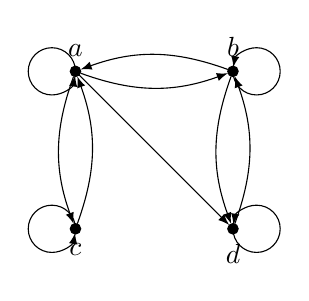
\begin{tikzpicture}
            \node (a) at (0, 2) [circle , draw, fill = black, label=above:$a$, scale = 0.4pt] {};
            \node (b) at (2, 2) [circle , draw, fill = black, label=above:$b$, scale = 0.4pt] {};
            \node (c) at (0, 0) [circle , draw, fill = black, label=below:$c$, scale = 0.4pt] {};
            \node (d) at (2, 0) [circle , draw, fill = black, label=below:$d$, scale = 0.4pt] {};
            \draw [-latex, bend right = 20] (a) edge (b);
            \draw [-latex, bend right = 20] (b) edge (a);
            \draw [-latex, bend right = 20] (a) edge (c);
            \draw [-latex, bend right = 20] (c) edge (a);
            \draw [-latex, bend right = 20] (d) edge (b);
            \draw [-latex, bend right = 20] (b) edge (d);
            \draw [-latex] (a) edge (d);
            \draw [-latex] (a) arc (0: 350: 0.3);
            \draw [] (b) arc (180: 360: 0.3);
            \draw [-latex] (2.6, 2) arc (0: 170: 0.3);
            \draw [-latex] (c) arc (0: 350: 0.3);
            \draw [] (d) arc (180: 360: 0.3);
            \draw [-latex] (2.6, 0) arc (0: 170: 0.3);
        \end{tikzpicture}
    \subsection*{4.7}
        The symmetric closure of $R$ is $R \cup R^{-1}$, as $M_{R \cup R^{-1}} = M_R \vee M_R^t$.
    \subsection*{4.9}
        \begin{itemize}
            \item [\textbf{a)}] 
                $\left\{
                    (1, 1), (1, 5),
                    (2, 3),
                    (3, 1), (3, 2), (3, 3), (3, 4),
                    (4, 1), (4, 5),
                    (5, 3), (5, 4)
                \right\}$
            \item [\textbf{b)}] 
                $\left\{
                    (1, 1), (1, 2), (1, 3), (1, 4),
                    (2, 1), (2, 5),
                    (3, 1), (3, 3), (3, 4), (3, 5),
                    (4, 1), (4, 2), (4, 3), (4, 4),
                    (5, 1), (5, 3), (5, 5)
                \right\}$
            \item [\textbf{f)}] $\left\{(a, b) \mid a,b \in \left[1, 5\right] \cap \mathbb{Z}\right\}$
        \end{itemize}
\end{document}